\PassOptionsToPackage{unicode}{hyperref}

%Präsentationsmodus:
%\documentclass[aspectratio=1610, professionalfonts, 9pt]{beamer}

%Druckmodus:
\documentclass[aspectratio=1610, professionalfonts, 9pt]{beamer}
%\usepackage[usenames,dvipsnames]{xcolor}
\usefonttheme[onlymath]{serif}
\usetheme[showtotalframes]{tudoflw}
\setbeamertemplate{bibliography item}{\insertbiblabel}
\ifluatex
  \usepackage{polyglossia}
  \setmainlanguage{german}
\else
  \ifxetex
    \usepackage{polyglossia}
    \setmainlanguage{german}
  \else
    \usepackage[german]{babel}
  \fi
\fi
    
% Mathematik
\usepackage{amsmath}
\usepackage{amssymb}
\usepackage{animate}
\usepackage{mathtools}
\usepackage{cancel}
\usepackage{xcolor}
\definecolor{tugreen}{HTML}{84b819}
\usepackage{hyperref}
\usepackage{bookmark}
\usepackage{verbatim}
\usepackage[]{algorithm2e}
\usepackage{pgf,tikz}
\usepackage{pgfplots}
\usetikzlibrary{arrows}
\usepackage{multirow}
\usepackage{ulem}
\usepackage{caption}
\usepackage{subcaption}
\usepackage[backend=biber]{biblatex}
\bibliography{LDV-Quellen}

\SetKw{Parameters}{Parameters}

\definecolor{wqwqwq}{rgb}{0.3764705882352941,0.3764705882352941,0.3764705882352941}
\definecolor{ududff}{rgb}{0.30196078431372547,0.30196078431372547,1.}
\definecolor{ffqqqq}{rgb}{1.,0.,0.}
%\usepackage[numbers]{natbib}

\DeclareMathOperator*{\argmax}{arg\,max}
\DeclareMathOperator*{\argmin}{arg\,min}

%%%%%%%%%%%%%%%%%%%%%%%%%%%%%%%%%%%%%%%%%%%%%%%%%%%%%%%%%%%%%%%%%%%%%%%%%%%%%%%%
%%%%%							Axel Krüger	   							   %%%%%
%%%%%							TU Dortmund								   %%%%%
%%%%%					Lehrstuhl für Förder- und Lagerwesen			   %%%%%
%%%%%					Logistische Datenverarbeitung					   %%%%%
%%%%% 						Sommersemester 2019							   %%%%%
%%%%%%%%%%%%%%%%%%%%%%%%%%%%%%%%%%%%%%%%%%%%%%%%%%%%%%%%%%%%%%%%%%%%%%%%%%%%%%%%

%Titel:
\title[MPC-Planner]{MPC Planner for mobile robots in Complex Environment}
%Autor
\author[A.~Abouelkhair]{Abdulrahman Abouelkhair\\ Supervised by: Mojtaba MasoudiNejad, M.Sc.}
%Lehrstuhl/Fakultät
\institute[FLW]{\small Lehrstuhl für Förder- und Lagerwesen \\  Fakultät Maschinenbau}
%Titelgrafik 
\titlegraphic{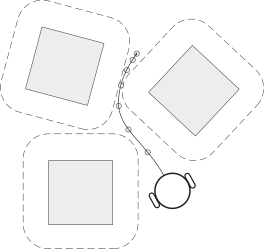
\includegraphics[width=0.3\textwidth]{pictures/mpc_robot}}
\date[SoSe 2019]{Master Thesis - Automation \& Robotics}


\AtBeginSection[]{
  \begin{frame}
  \vfill
  \centering
  \begin{beamercolorbox}[sep=8pt,center,shadow=false,rounded=true]{title in head/foot}
    \setlength{\fboxrule}{1pt}
    \fcolorbox{tugreen}{white}{\usebeamerfont{title}\insertsectionhead\par}
  \end{beamercolorbox}
  \vfill
  \end{frame}
}

 %Damit das Inhaltsverzeichnis nummeriert ist
\setbeamertemplate{sections/subsections in toc}[sections numbered]
\setbeamertemplate{subsection in toc}[subsections numbered]


\begin{document}

\maketitle

\begin{frame}
    \frametitle{Agenda}
    %\tableofcontents[pausesections]
    \tableofcontents
\end{frame}

% Organisatorisches
\section*{Organisatorisches}

	\begin{frame}
		\frametitle{Kontakt}
		\begin{tabular}{ll}
			Anschrift & Technische Universität Dortmund\\
			& Lehrstuhl für Förder- und Lagerwesen (FLW)\\
			& LogistikCampus\\
			& Joseph-von-Fraunhofer-Str. 2-4 \\
			& 44227 Dortmund\\[0.1cm]
			Name & Mojtaba MasoudiNejad, M.Sc.\\[0.1cm]
			Raum& A4.06\\[0.1cm]
			Telefon& +49 231 755-3236\\[0.1cm]
			Mail& mojtaba.masoudinejad@tu-dortmund.de\\[0.1cm]
			Sprechstunde& flexibel nach Vereinbarung\\[0.1cm]
		\end{tabular}
	\end{frame}

	\begin{frame}
		\frametitle{Master Präsentation Termine}
		\begin{tabular}{ll}
		Ort & FLW / A3.16\\[0.1cm]
		Zeit & 18 Oct. 2019 um 11:00 - 11:25 \\[0.1cm]
		Examiners &  Moritz Roidl, Dipl.-Inform.\\
		&Mojtaba MasoudiNejad, M.Sc.
		\end{tabular}\\[1cm]
	\end{frame}

	\begin{frame}
	\frametitle{Literatur}
	    \begin{columns}[T]
	        \begin{column}{0.49\textwidth}
	            \begin{itemize}%[<+->] Kommentar entfernen falls jeder Punkt einzeln erscheinen soll
					\item Title: Springer Handbook of Robotics
					\item Author: Khatib, Oussama ; Siciliano, Bruno
					\item Link: \href{https://www.ub.tu-dortmund.de/katalog/titel/HT019024543}{https://www.ub.tu-dortmund.de/katalog/titel/HT019024543}
	        	\end{itemize}
	        \end{column}
	        \begin{column}{0.49\textwidth}
	        	\centering
	            \includegraphics[scale=0.25]{pictures/springer_robotics.pdf}
	        \end{column}
	    \end{columns}
	\end{frame}

	\begin{frame}
		\frametitle{Literatur}
		\begin{columns}[T]
			\begin{column}{0.49\textwidth}
				\begin{itemize}%[<+->] Kommentar entfernen falls jeder Punkt einzeln erscheinen soll
					\item Title: Model Predictive Control : Theory, Computation, and Design 
					\item Author: Diehl, Moritz ; Mayne, David Q ; Rawlings, James Blake
					\item Link: \href{https://www.ub.tu-dortmund.de/katalog/titel/HT019602243}{https://www.ub.tu-dortmund.de/katalog/titel/HT019602243}
				\end{itemize}
			\end{column}
			\begin{column}{0.49\textwidth}
				\centering
				\includegraphics[scale=0.305]{pictures/mpc_book_cover.png}
			\end{column}
		\end{columns}
	\end{frame}

	\begin{frame}
		\frametitle{Literatur}
		\begin{columns}[T]
			\begin{column}{0.49\textwidth}
				\begin{itemize}%[<+->] Kommentar entfernen falls jeder Punkt einzeln erscheinen soll
					\item Title: Numerical Optimization
					\item Author: Nocedal, Jorge ; Wright, Stephen J
					\item Link: \href{https://www.ub.tu-dortmund.de/katalog/titel/HT014641035}{https://www.ub.tu-dortmund.de/katalog/titel/HT014641035}
				\end{itemize}
			\end{column}
			\begin{column}{0.49\textwidth}
				\centering
				\includegraphics[scale=0.2]{pictures/numerical_optimization.png}
			\end{column}
		\end{columns}
	\end{frame}

% Ziele
\section*{Ziele}
\begin{frame}
\frametitle{Lernziele}
Am Ende des Semesters können Sie
\begin{itemize}
\item die Grundbegriffe der Statistik unterscheiden und erläutern,
\pause
\item grundlegende statistische und wahrscheinlichkeitstheoretische Kennzahlen bestimmen und interpretieren,
\pause
\item ausgewählte maschinelle Lernverfahren in ihren Grundzügen erklären und einsetzen,
\pause
\item Aufgabentypen des maschinellen Lernens unterscheiden und für den jeweiligen Aufgabentyp geeignete Verfahren benennen,
\pause
\item erlernte Modelle validieren und testen,
\pause
\item Ergebnisse der Datenanalyse visualisieren,
\pause
\item die Anforderungen an ein Datenbanksystem benennen und erläutern.
\end{itemize}
\end{frame}
%\begin{frame}
%\frametitle{Der rote Faden}
%% Für Bilder Argument T benutzen:
%    \begin{columns}[T]
%        \begin{column}{0.49\textwidth}
%            \begin{itemize}%[<+->] Kommentar entfernen falls jeder Punkt einzeln erscheinen soll
%            	\item[$\,\blacktriangleright$] Daten aufnehmen
%            	\begin{itemize}
%            		\item Was sind Daten?
%            		\item Woher kommen Daten?
%            	\end{itemize}	
%            	\item[$\,\blacktriangleright$] Daten speichern
%            		\begin{itemize}
%            			\item Welche Anforderungen gibt es an Datenbanken?
%            			\item Wie kann ich Daten in einer relationalen Datenbank abrufen?
%            		\end{itemize}
%            	\item[$\,\blacktriangleright$] Daten auswerten
%            	\begin{itemize}
%            		\item Welche Möglichkeiten zur Auswertung gibt es?
%            		\item Was ist maschinelles Lernen und was sind die Einsatzmöglichkeiten?
%            		\item Wie prüfe ich ein erlerntes Modell?
%            		\item Wie kann ich Ergebnisse visualisieren?
%            	\end{itemize}
%        	\end{itemize}
%        \end{column}
%        \begin{column}{0.49\textwidth}
%            \includegraphics[width=\textwidth]{images/roter-faden.jpg}
%        \end{column}
%    \end{columns}
%\end{frame}

% Einführung
\section{Introduction and Motivation}

	\begin{frame}
		\frametitle{Introduction}
		\begin{columns}
			\begin{column}{0.49\textwidth}
				\begin{itemize}
					\item \onslide<1->{Novel Strategy} \\[0.7cm]
					\item \onslide<2->{Decentralized Navigation} \\[0.7cm]
					\item \onslide<3->{Optimal Motion Planning} \\[0.7cm]
					\item \onslide<5->{Autonomous Decision Making}
				\end{itemize}
			\end{column}
			\pause
			\begin{column}{0.49\textwidth}
				\centering
				\onslide<4->{\includegraphics[width=0.85\textwidth]{pictures/robot_comic.png}}
			\end{column}
		\end{columns}
	\end{frame}
	
	\begin{frame}
		\frametitle{Latest Approaches and Motivation}
	    \begin{columns}[T]
	        \begin{column}{0.49\textwidth}
	            \begin{itemize}%[<+->] Kommentar entfernen falls jeder Punkt einzeln erscheinen soll
					\item \onslide<1->{Environment Previous Knowledge}\\[0.5cm]
					\item \onslide<3->{Maximum speed $\leq 1.5 m/s$} \\[1cm]
					\item \onslide<4->{This approach has the potential to improve : \\[0.5cm]
					\begin{itemize}
						\item system performance \\[0.2cm]
						\item fast path towards goal
					\end{itemize}
					}
	        	\end{itemize}
	        \end{column}
	        \begin{column}{0.49\textwidth}
	        	\begin{itemize}%[<+->] Kommentar entfernen falls jeder Punkt einzeln erscheinen soll
	        		\item \onslide<2->{Global Planner}
	        	\end{itemize}
        		\centering
        		\only<1>{\includegraphics[width=0.8\textwidth]{pictures/figure_1.png}}
        		\only<2>{\includegraphics[width=0.8\textwidth]{pictures/figure_2.png}}
        		\only<3->{\includegraphics[width=0.8\textwidth]{pictures/figure.png}}
	        \end{column}
	    \end{columns}
	\end{frame}
	
	\begin{frame}
		\begin{block}{Proposed Approach\footnotemark}
			\begin{itemize}
				\pause
				\item On-line trajectory planning \\ [0.4cm]
				\pause
				\item Without \textit{global planner} \\ [0.4cm]
				\pause
				\item Without \textit{map} \\ [0.4cm]
				\pause
				\item Dynamic Environment, e.g. \textit{(pedestrian, multi-robots)} \\ [0.4cm]
				\pause
				\item Robot speed $> 1.5 m/s$ \\ [0.4cm]
				\pause
				\item Smooth navigation \\ [0.4cm]
				\pause
				\item Deadlock free
			\end{itemize}
		\end{block}
		\footnotetext[1]{
			Hoy, Michael and Matveev, Alexey S. and Savkin, Andrey V. 
			\say{
				\href{https://www.cambridge.org/core/journals/robotica/article/algorithms-for-collisionfree-navigation-of-mobile-robots-in-complex-cluttered-environments-a-survey/ADA8F6F7E30123629A26B08DA0C79C8C}{
					\textcolor{tudark}{Algorithms for collision-free navigation of mobile robots in complex cluttered environments: a survey}
				}
			}. In Cambridge University Press (2016).
		}
	\end{frame}

	\begin{frame}
		\begin{columns}[T]
			\begin{column}{0.49\textwidth}
			\begin{itemize}%[<+->] Kommentar entfernen falls jeder Punkt einzeln erscheinen soll
				\item Current Approach: \\[0.2cm]
				\begin{itemize}
					\item Laser Scanner + Map \\[0.1cm]
					\item Robot's estimated location 
				\end{itemize}
			\end{itemize}
			\includegraphics[scale=0.67]{pictures/navigation_ros_2.pdf}
			\end{column}
			\pause
			\begin{column}{0.49\textwidth}
				\begin{itemize}%[<+->] Kommentar entfernen falls jeder Punkt einzeln erscheinen soll
					\item Proposed Approach: \\[0.2cm]
					\begin{itemize}
						\item Robot localization \\[0.1cm]
						\item Obstacles location 
					\end{itemize}
				\end{itemize}
				\includegraphics[scale=0.75]{pictures/navigation_ros_3.pdf}
			\end{column}
		\end{columns}
	\end{frame}

	\begin{frame}
		\frametitle{Model Predictive Control}
		\centering
		\only<1>{\animategraphics[loop,controls,width=0.75\textwidth]{2}{pictures/mpc_group/MPC_scheme_basic-}{0}{6}}
		\only<2>{\includegraphics[scale=1.0]{pictures/mpc_group/MPC_scheme_basic-7.pdf}}
	\end{frame}

	\begin{frame}
		\frametitle{On-line Trajectory (prediction horizon)}
		\centering
		\movie[width=0.42\textwidth, height=0.45\textwidth]
		{\includegraphics[width=0.42\textwidth]{pictures/path.png}}{videos/path.mov}
	\end{frame}

	\begin{frame}
		\frametitle{NMPC Optimization Problem Schematic}
		\centering
		\only<1>{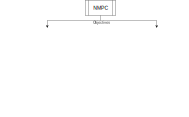
\includegraphics[scale=0.8]{pictures/mpc_planner_group/mpc_planner_0.pdf}}
		\centering
		\only<2>{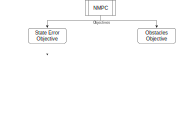
\includegraphics[scale=0.8]{pictures/mpc_planner_group/mpc_planner_1.pdf}}
		\centering
		\only<3>{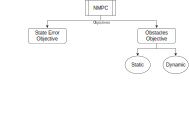
\includegraphics[scale=0.8]{pictures/mpc_planner_group/mpc_planner_2.pdf}}
		\centering
		\only<4>{\includegraphics[scale=0.8]{pictures/mpc_planner_group/mpc_planner_3.pdf}}
		\centering
		\only<5>{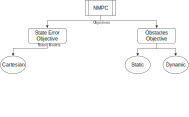
\includegraphics[scale=0.8]{pictures/mpc_planner_group/mpc_planner_4.pdf}}
		\centering
		\only<6>{\includegraphics[scale=0.8]{pictures/mpc_planner_group/mpc_planner_5.pdf}}
		\centering
		\only<7>{\includegraphics[scale=0.8]{pictures/mpc_planner_group/mpc_planner_6.pdf}}
	\end{frame}

% Statistik
\section{Obstacles Formulation}

	\begin{frame}
		\frametitle{Robot Environment}
		\begin{columns}[T]
			\begin{column}{0.3\textwidth}
				\begin{itemize}
					\item Static obstacles location \\[1.0cm]
					\item Dynamic obstacles trajectory
				\end{itemize}
			\end{column}
			\begin{column}{0.7\textwidth}
				\centering
				\animategraphics[loop,controls,width=0.7\linewidth]{2}{pictures/robot_env_group/robot_env-}{0}{8}
				%\includegraphics[scale=0.7]{pictures/robot_env.pdf}
			\end{column}
		\end{columns}
	\end{frame}

	\begin{frame}
		\frametitle{Laser Scanner}
		\begin{columns}[T]
			\begin{column}{0.42\textwidth}
				\centering
				\onslide<1->{\includegraphics[scale=0.45]{pictures/laser_ranges.pdf}}
				\onslide<2->{
				\begin{block}{Laser scanner message}
					\[\overrightarrow{data}(k) = \left\{
					\begin{array}{lr}
					angle_{min} \\
					angle_{max} \\
					\overrightarrow{angle}_{inc}, \quad \qquad \forall \enspace \delta \in \overrightarrow{angle}_{inc} \\
					range_{min} \\
					range_{max} \\
					\overrightarrow{ranges}, \qquad \qquad \forall \enspace \sigma \in \overrightarrow{ranges}
					\end{array}
					\right.
					\]
				\end{block}
				}
			\end{column}
			\begin{column}{0.52\textwidth}
				\centering
				 \onslide<3->{\includegraphics[scale=0.51]{pictures/robot_laser.pdf}}
			\end{column}
		\end{columns}
	\end{frame}

	\begin{frame}
		\frametitle{Homogeneous Transformation}
		\begin{columns}[T]
			\begin{column}{0.4\textwidth}
				\onslide<2->{
				\begin{block}{Rotation Matrix regarding $Z$-axis}
					\[
						T_z = 
						\begin{pmatrix}
							\cos\theta_z & -\sin\theta_z & 0 & x_{trns} \\
							\sin\theta_z &  \cos\theta_z & 0 & y_{trns}  \\
							0		   & 0 			 & 1 & y_{trns}  \\
							0		   & 0			 & 0 & 1 \\
						\end{pmatrix}
					\]
				\end{block}
				}
				\onslide<3->{
				\begin{block}{Co-ordinate Transformation}
					\[
						T_{obst\_map} = 
						T_{ft\_map} T_{r\_ft} T_{lsr\_r}
						\begin{pmatrix}
							x_{obst} \\
							y_{obst} \\
							z_{obst} \\
							1 
						\end{pmatrix}
					\]
				\end{block}
				}
			\end{column}
			\begin{column}{0.55\textwidth}
				\centering
				\onslide<1->{\includegraphics[scale=0.9]{pictures/laser_robot_frame.pdf}}
			\end{column}
		\end{columns}
	\end{frame}

	\begin{frame}
		\frametitle{Homogeneous Transformation}
		\begin{columns}[T]
			\begin{column}{0.49\textwidth}
				\begin{itemize}
					\item $
					T_{footprint\_map} \enspace \text{ }=
					\begin{pmatrix}
						\cos\theta_r & -\sin\theta_r & 0 & x_{r} \\
						\sin\theta_r & \cos\theta_r & 0 & y_{r} \\
						0 & 0 & 1 & 0 \\
						0 & 0 & 0 & 1 \\
					\end{pmatrix}
					$
					\item $
					T_{robot\_footprint} \enspace= 
					\begin{pmatrix}
						1 & 0 & 0 & 0 \\
						0 & 1 & 0 & 0 \\
						0 & 0 & 1 & -0.125 \\
						0 & 0 & 0 & 1 \\
					\end{pmatrix}
					$
					\item $
					T_{laser\_robot} \qquad= 
					\begin{pmatrix}
						1 & 0 & 0 & 0 \\
						0 & 1 & 0 & -0.245 \\
						0 & 0 & 1 & -0.051 \\
						0 & 0 & 0 & 1 \\
					\end{pmatrix}
					$
				\end{itemize}
			\end{column}
			\begin{column}{0.49\textwidth}
				\centering
				\includegraphics[scale=0.5]{pictures/robotnik.pdf}
			\end{column}
		\end{columns}
	\end{frame}

	\begin{frame}
		\frametitle{Saved Obstacles Frame}
		\centering
		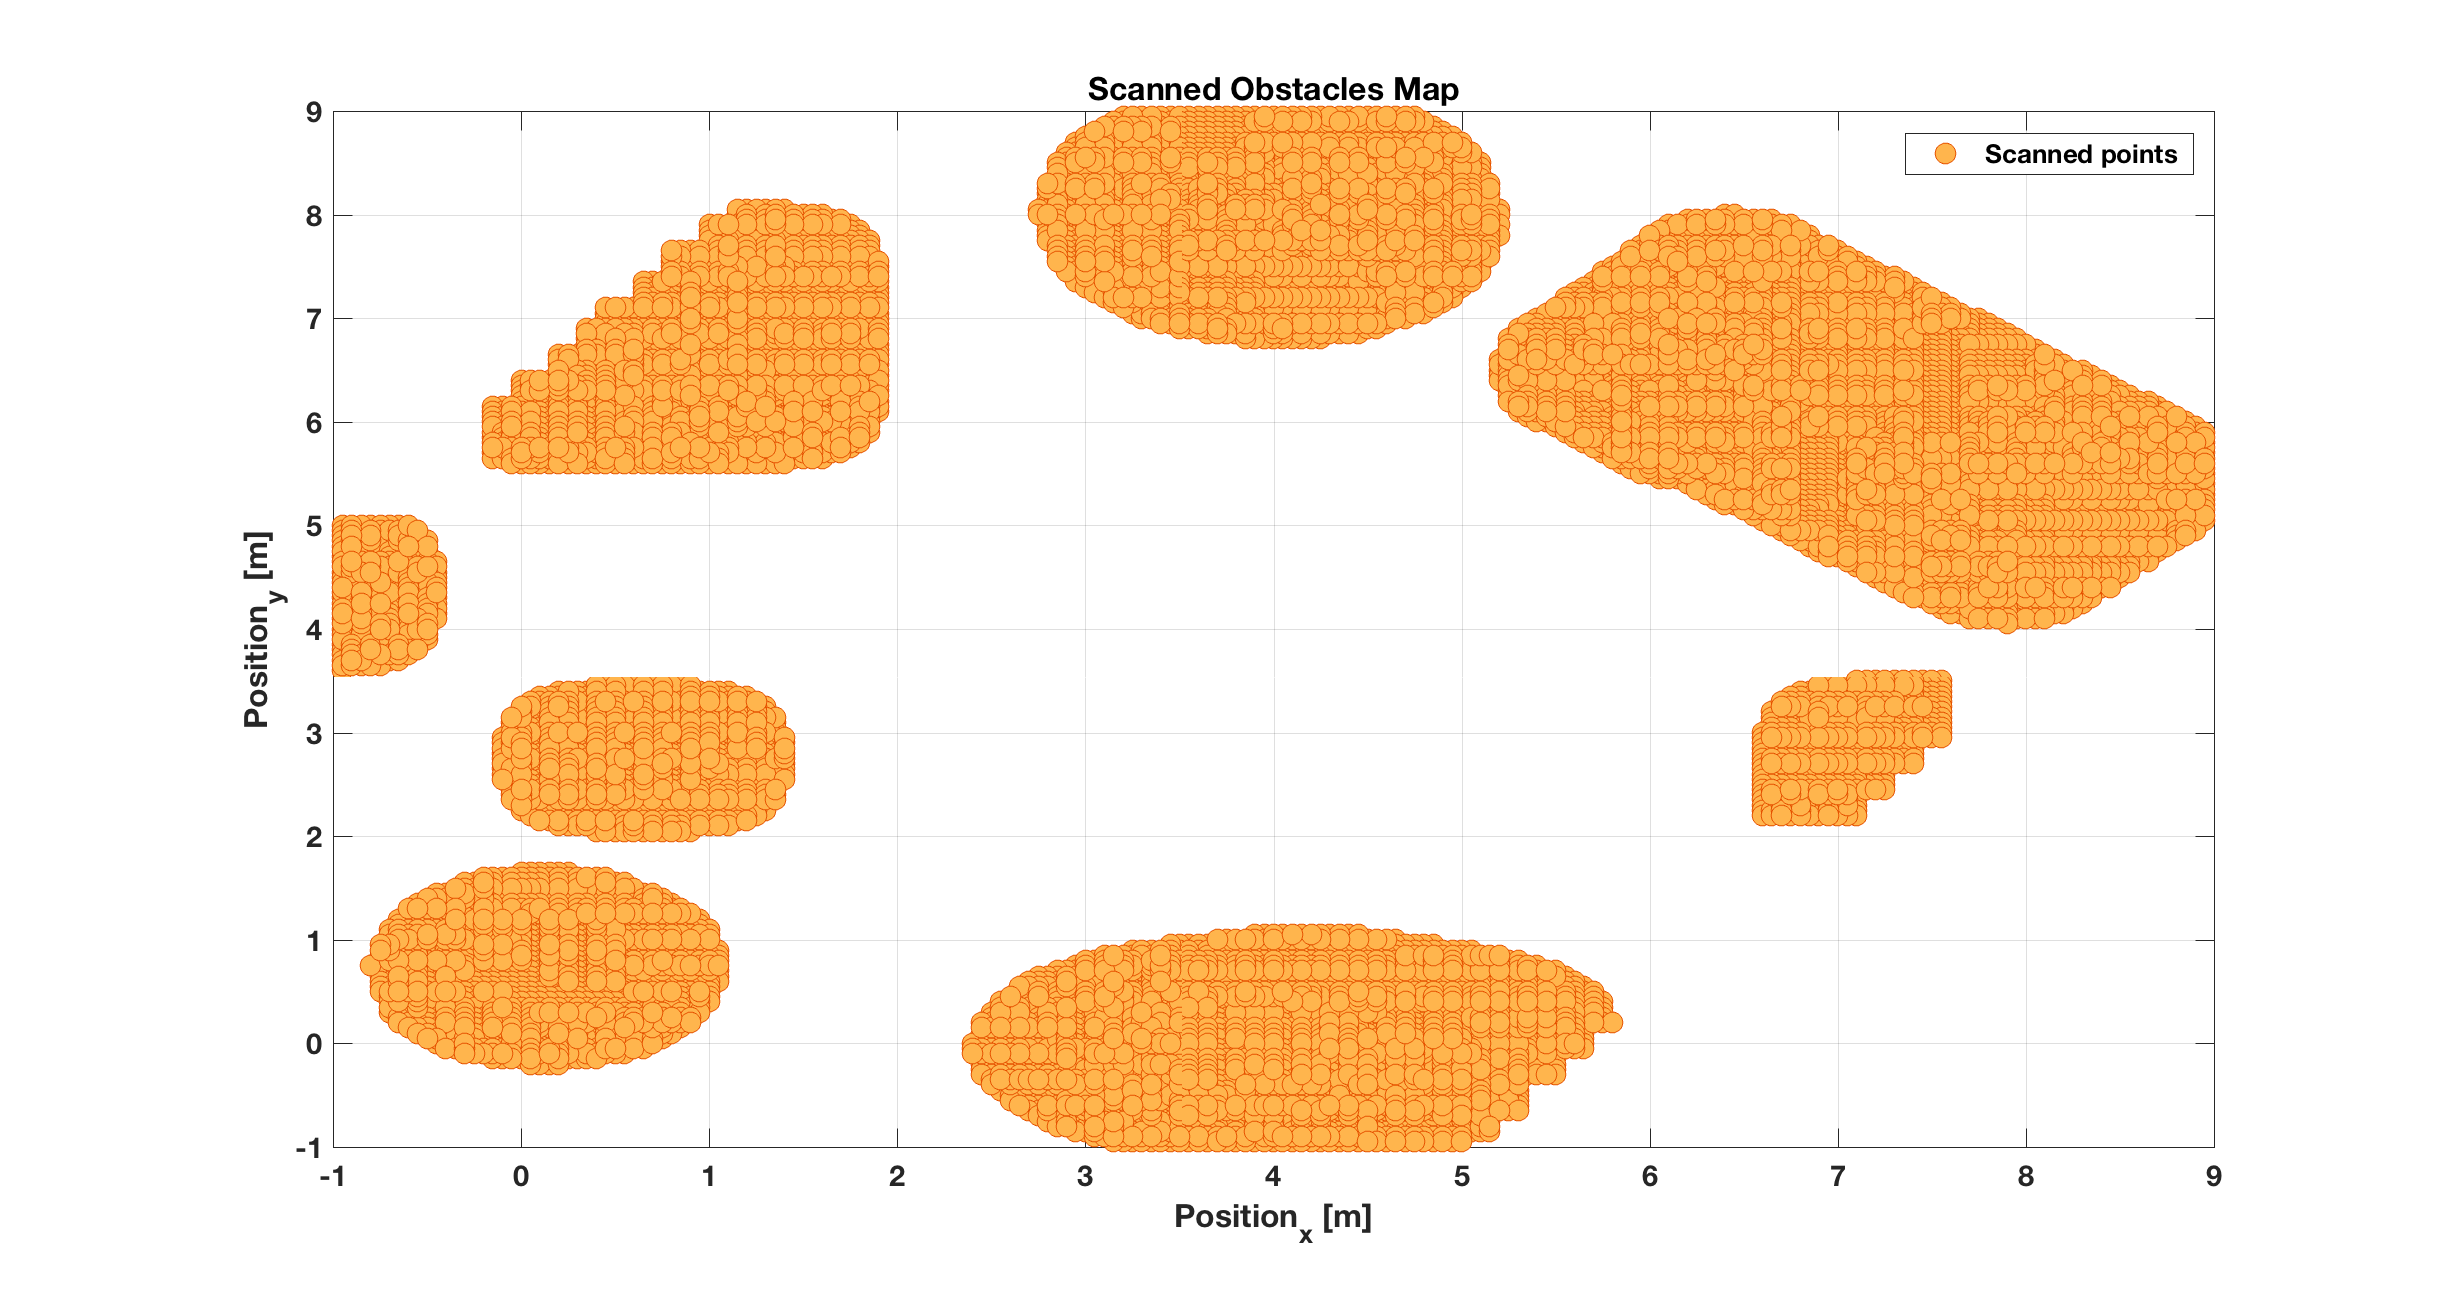
\includegraphics[scale=0.46]{pictures/intial_map.eps}
	\end{frame}

	\begin{frame}
		\frametitle{Cluster + Fitting Algorithm}
		\onslide<1->{
		\begin{block}{Density-Based Spatial Clustering of Applications with Noise (DBSCAN)}
			Statistical search algorithm
		\end{block}
		\begin{block}{Least Square Fitting Ellipse (LSFE)}
			Numerical fitting algorithm for each set of data.
		\end{block}
		}
		\begin{columns}[T]
			\onslide<2->{
			\begin{column}{0.32\textwidth}
				\begin{itemize}
					\item Edged data points
				\end{itemize}
				\includegraphics[scale=0.65]{pictures/lsellipse1.pdf}
			\end{column}
			}
			\onslide<3->{
			\begin{column}{0.32\textwidth}
				\begin{itemize}
					\item Concave data points
				\end{itemize}
				\includegraphics[scale=0.65]{pictures/lsellipse2.pdf}
			\end{column}
			}
			\onslide<4->{
			\begin{column}{0.32\textwidth}
				\begin{itemize}
					\item Lined-curved data points
				\end{itemize}
				\includegraphics[scale=0.65]{pictures/lsellipse3.pdf}
			\end{column}
			}
		\end{columns}
	\end{frame}

	\begin{frame}
		\frametitle{Fitted Frame}
		\centering
		\includegraphics[scale=0.13]{pictures/map_clustered.eps}
	\end{frame}

	\begin{frame}
		\frametitle{Dynamic Obstacles Tracking}
		\begin{columns}[T]
			\begin{column}{0.4\textwidth}
				\onslide<2->{
				\begin{block}{Dyn. obstacles estimation}
					\begin{align*}
						&\hat{\mathbf{x}}_{i,k} = 
						\begin{pmatrix}
							\hat{x}_{i,k} \\
							\hat{y}_{i,k} \\
							\hat{\theta}_{i,k}
						\end{pmatrix},
						\qquad \qquad \hat{\mathbf{x}}_{i,k} =
						\begin{pmatrix}
							\hat{v}_{i,k} \\
							\hat{\omega}_{i,k}
						\end{pmatrix}
						\\
						&\hat{\mathbf{X}}_{i,k} := \{ \hat{\mathbf{x}}_{i,k}, \hat{\mathbf{x}}_{i,k+1}, \cdots, \hat{\mathbf{x}}_{i,k+N_p} \} \\
						&\bar{\mathbf{X}}_{i,k} := \{ \bar{\mathbf{x}}_{i,k}, \bar{\mathbf{x}}_{i,k+1}, \cdots, \bar{\mathbf{x}}_{i,k+N_p}\}
					\end{align*}
				\end{block}
				}
				\onslide<3->{
				\begin{block}{Dynamic obstacles vector}
					\[
					\hat{\mathbf{Z}}_{i,k} = 
					\begin{cases}
						\hat{\mathbf{X}}_{i,k}, & \text{if } i \in I_{un} \\
						\bar{\mathbf{X}}_{i,k}, & \text{if } i \in I_{robots}.
					\end{cases}
					\]
				\end{block}
				}
			\end{column}
			\begin{column}{0.56\textwidth}
				\centering
				\onslide<1->{\includegraphics[scale=0.7]{pictures/robot_env_diff.pdf}}
			\end{column}
		\end{columns}
	\end{frame}

	\begin{frame}
		\frametitle{Obstacles Detection Block Diagram}
		\centering
		\includegraphics[scale=0.9]{pictures/block_diagram_obst_1.pdf}
	\end{frame}



% Julia
\section{Experiments}
	
	\begin{frame}
		\centering
		\only<1>{\includegraphics[scale=0.69]{pictures/eperiments_1.pdf}}
		\only<2>{\includegraphics[scale=0.69]{pictures/eperiments_2.pdf}}
		\only<3>{\includegraphics[scale=0.69]{pictures/eperiments_3.pdf}}
		\only<4>{\includegraphics[scale=0.69]{pictures/eperiments.pdf}}
	\end{frame}
 

% Datenanalyse
\section{Approach Upgrade}

	\begin{frame}
		\frametitle{NMPC with Switching Objective}
		\onslide<1->
		{
			\begin{block}{Optimization Problem}
				\parbox[c][3\baselineskip][t]{\textwidth}{
					\begin{align*}
					\underset{\vartheta^*,\mathbf{U}^*}{\text{min    }}
					J_{N_p}(\vartheta_k) = (1 - \tikzmark{a16}\beta_2 - \tikzmark{a17}\beta_3) \times J_1 + 
					\tikzmark{a18}\beta_2 \times J_2 - \tikzmark{a19}\beta_3 \times J_3
					\end{align*}
				}
			\end{block}
		}
		\onslide<3->
		{Objectives:}
		\begin{itemize}
			\onslide<4->
			{\item $J_1 = \ell_{p,1}(\cdot,\cdot)$}
			\onslide<5->
			{\item $J_2 = w_2 \times J_1 + J_4$}
			\onslide<6->
			{\item $J_3 = w_3 \times J_1 + J_5$ \\ [1cm]}
		\end{itemize}
		\onslide<7->
		{
			\[
			J_{N_p}(\vartheta_k) = 
			\begin{cases}
			\beta_2 = 0, \enspace \beta_3 = 1, 				& \text{if a dynaminc obstacle is detected} \\
			\beta_2 = 1, \enspace \beta_3 = 0, 				& \text{else, if the robot is near the goal} \\
			\beta_2 = 0, \enspace \beta_3 = 0, 				& \text{otherwise} 
			\end{cases}
			\]
		}
		\begin{tikzpicture}[overlay, remember picture]
		\coordinate (A16) at ($({pic cs:a16})+(1ex, 0.5ex)$);
		\coordinate (A17) at ($({pic cs:a17})+(1ex, 0.5ex)$);
		\coordinate (A18) at ($({pic cs:a18})+(1ex, 0.5ex)$);
		\coordinate (A19) at ($({pic cs:a19})+(1ex, 0.5ex)$);
		\onslide<2->{
			\node [fit=(A16), draw=tugreen, circle, thick, inner sep=4.5pt] (n16) {};
			\node [fit=(A17), draw=tugreen, circle, thick, inner sep=4.5pt] (n17) {};
			\node [fit=(A18), draw=tugreen, circle, thick, inner sep=4.5pt] (n18) {};
			\node [fit=(A19), draw=tugreen, circle, thick, inner sep=4.5pt] (n19) {};
			\node[overlay, below of= n16, node distance = 4em] at (8.5,5) (t16) {Binary};
			\node[overlay, below of= t16, node distance = 1em] (t16_1) {Multipliers};
			\draw [thick, -latex, tugreen] (n16.south) to [above] (t16.north);
			\draw [thick, -latex, tugreen] (n17.south) to [above] (t16.north);
			\draw [thick, -latex, tugreen] (n18.south) to [above] (t16.north);
			\draw [thick, -latex, tugreen] (n19.south) to [above] (t16.north);
		}
		\end{tikzpicture}
	\end{frame}
	
	\begin{frame}
		\frametitle{NMPC with Switching Objective Block Diagram}
		\begin{figure}[hbtp]
			\centering
			\includegraphics[scale=0.65]{pictures/block_diagram_polar_switch_1.pdf}
			\caption{NMPC Control Loop with Switching Objective}
		\end{figure}
	\end{frame}

	\begin{frame}
		\frametitle{Scenario \textrm{IV}: Dynamic Environment}
		\begin{figure}[hbtp]
			\centering
			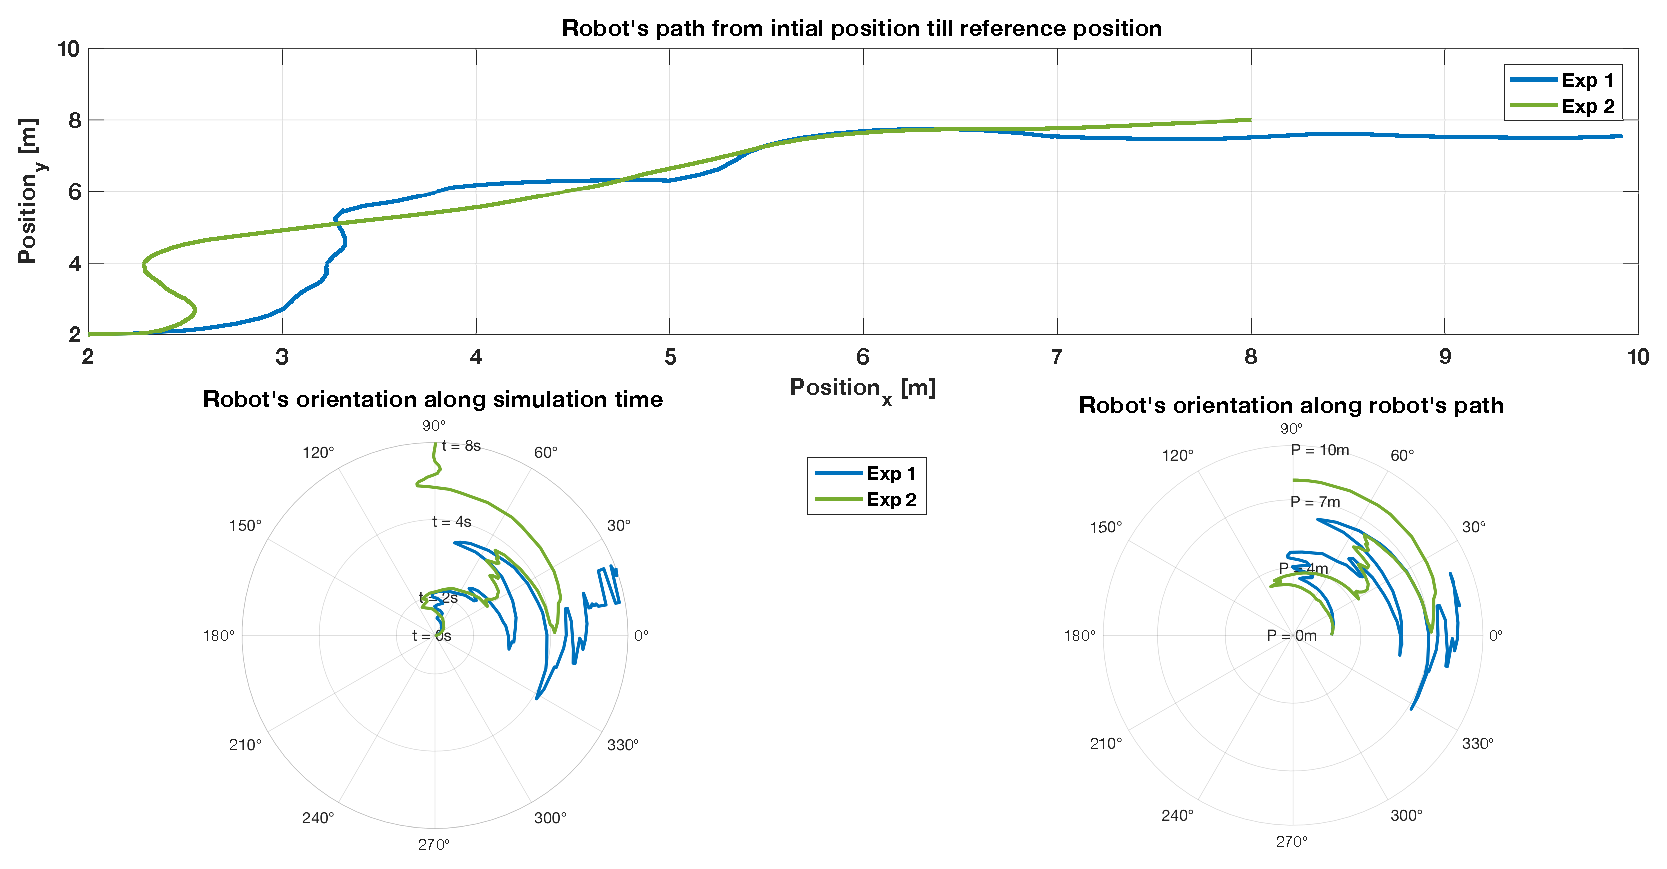
\includegraphics[scale=0.44]{pictures/graphs/sn3_states.eps}
			\caption{State Trajectory Evolution}
		\end{figure}
	\end{frame}
	
	\begin{frame}
		\frametitle{Scenario \textrm{IV}: Dynamic Environment}
		\begin{figure}[hbtp]
			\centering
			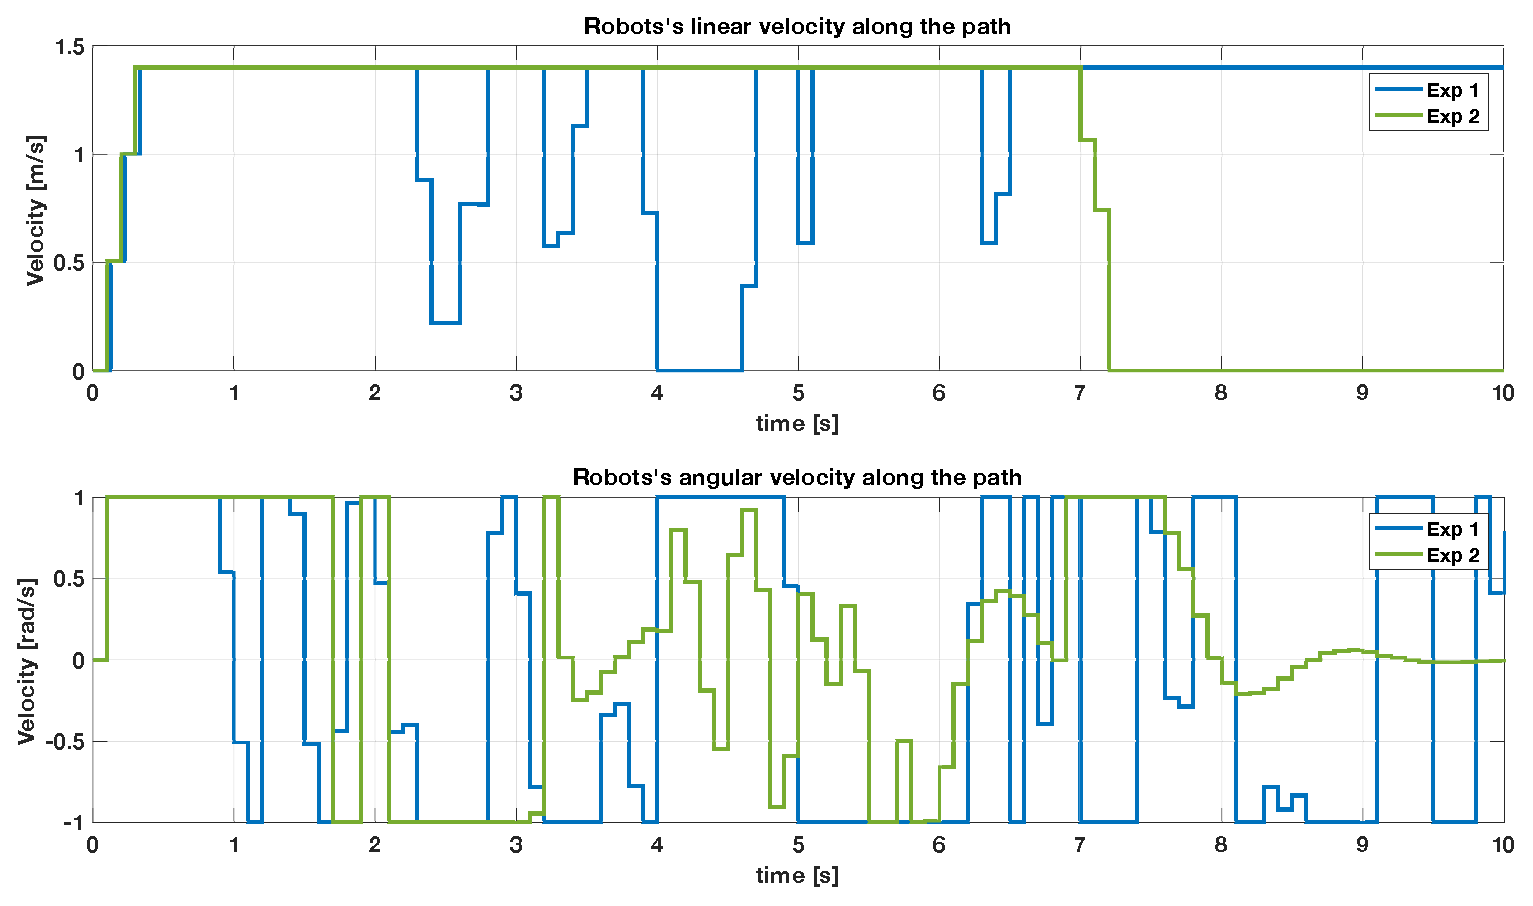
\includegraphics[scale=0.42]{pictures/graphs/sn3_inputs.eps}
			\caption{Input Trajectory Evolution}
		\end{figure}
	\end{frame}
	
	\begin{frame}
		\frametitle{Scenario \textrm{IV}: Dynamic Environment}
		\begin{figure}[hbtp]
			\centering
			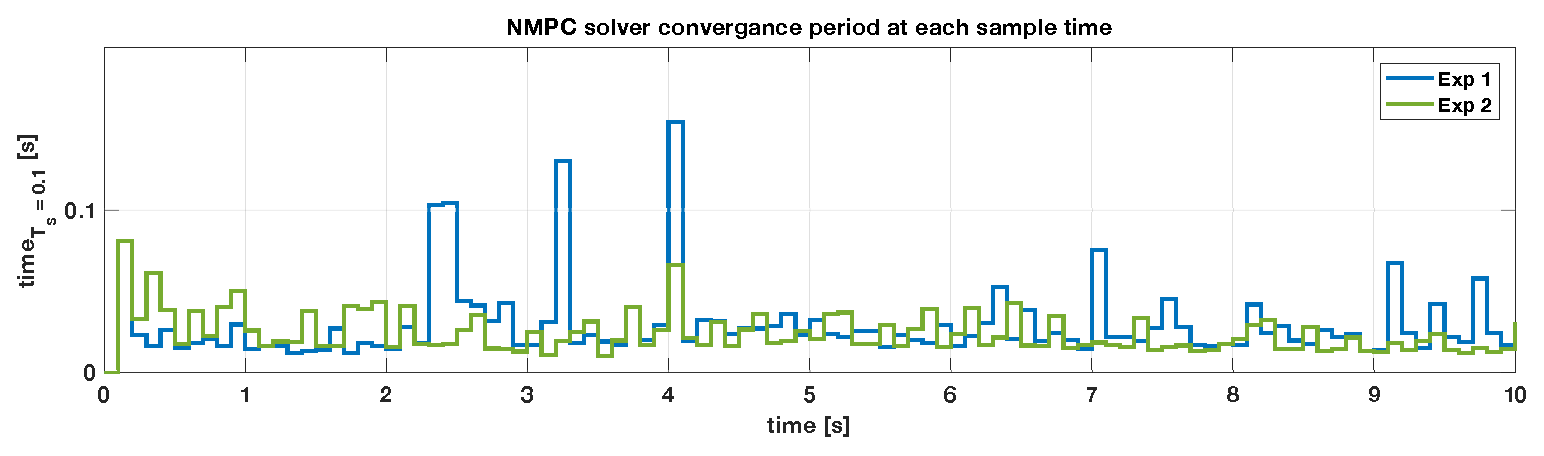
\includegraphics[scale=0.42]{pictures/graphs/sn3_solver_time.eps}
			\caption{NMPC Computational Effort}
		\end{figure}
	\end{frame}
	
	\begin{frame}
		\frametitle{Scenario \textrm{IV}: Dynamic Environment}
		\centering
		\movie[width=0.451\textwidth, height=0.865\textheight]
		{\includegraphics[width=0.45\textwidth]{pictures/good_1.png}}{videos/good_1.mov}
		\nocite{hoy_matveev_savkin_2015}
	\end{frame}

% Datenbanken
% \section{Datenbanken}
\begin{frame}
\frametitle{Relation}
\begin{block}{Def.: Relation}
Eine Menge $R$ heißt $n$-stellige (auch $n$-äre) Relation über Mengen $A_1,A_2,\ldots,A_n$, falls
\begin{equation*}
R \subseteq \{ (x_1,x_2,\ldots, x_n) | x_1 \in A_1 \text{ und } x_2\in A_2 \text{ und  } \ldots \text{ und } x_n \in A_n \}
\end{equation*}
gilt.
\end{block}
Anmerkungen:\\
\begin{itemize}
\item Eine Relation $R$ ist eine Menge von Tupeln
\item Die $i$-te Komponente eines Tupels ist ein Element von $A_i$
\end{itemize}
\end{frame}
\begin{frame}
\frametitle{Beispiel zur Relation}
Es sei
\begin{itemize}
\item $A_1 = \{ \text{Nudeln, Ketchup, Eier }\}$
\item $A_2 = \mathbb{N}_0$
\item $A_3 = \mathbb{R}_{\geq 0}$
\end{itemize}
\pause
Eine Relation $R$ über $A_1,A_2,A_3$ ist etwa
\begin{equation*}
R = \{(\text{Nudeln}, 3, 0.9),(\text{Ketchup}, 1, 1.50),(\text{Eier}, 2, 1.99) \}.
\end{equation*}
Hier ist $R$ eine Bestandsliste der Lebensmittel mit Einkaufspreisen in einer Studenten-WG, z.B. sind drei Nudelpackungen zu einem Einkaufspreis von je 0,90 € vorhanden.
\end{frame}

%Quellenverzeichnis
\begin{frame}[allowframebreaks]
        \frametitle{Quellenverzeichnis}
        %\bibliographystyle{plain}
        \printbibliography
\end{frame}
\end{document}
